%%%%%%%%%%%%%%%%%%%%%%%%%%%%%%%%%%%%%%%%%%%%%%%%%%%%%%%%%%%%%%%%%%%%%%%%%%%%%%%%
\section{Supplementary materials}
%%%%%%%%%%%%%%%%%%%%%%%%%%%%%%%%%%%%%%%%%%%%%%%%%%%%%%%%%%%%%%%%%%%%%%%%%%%%%%%%

\begin{figure}[!htbp]
  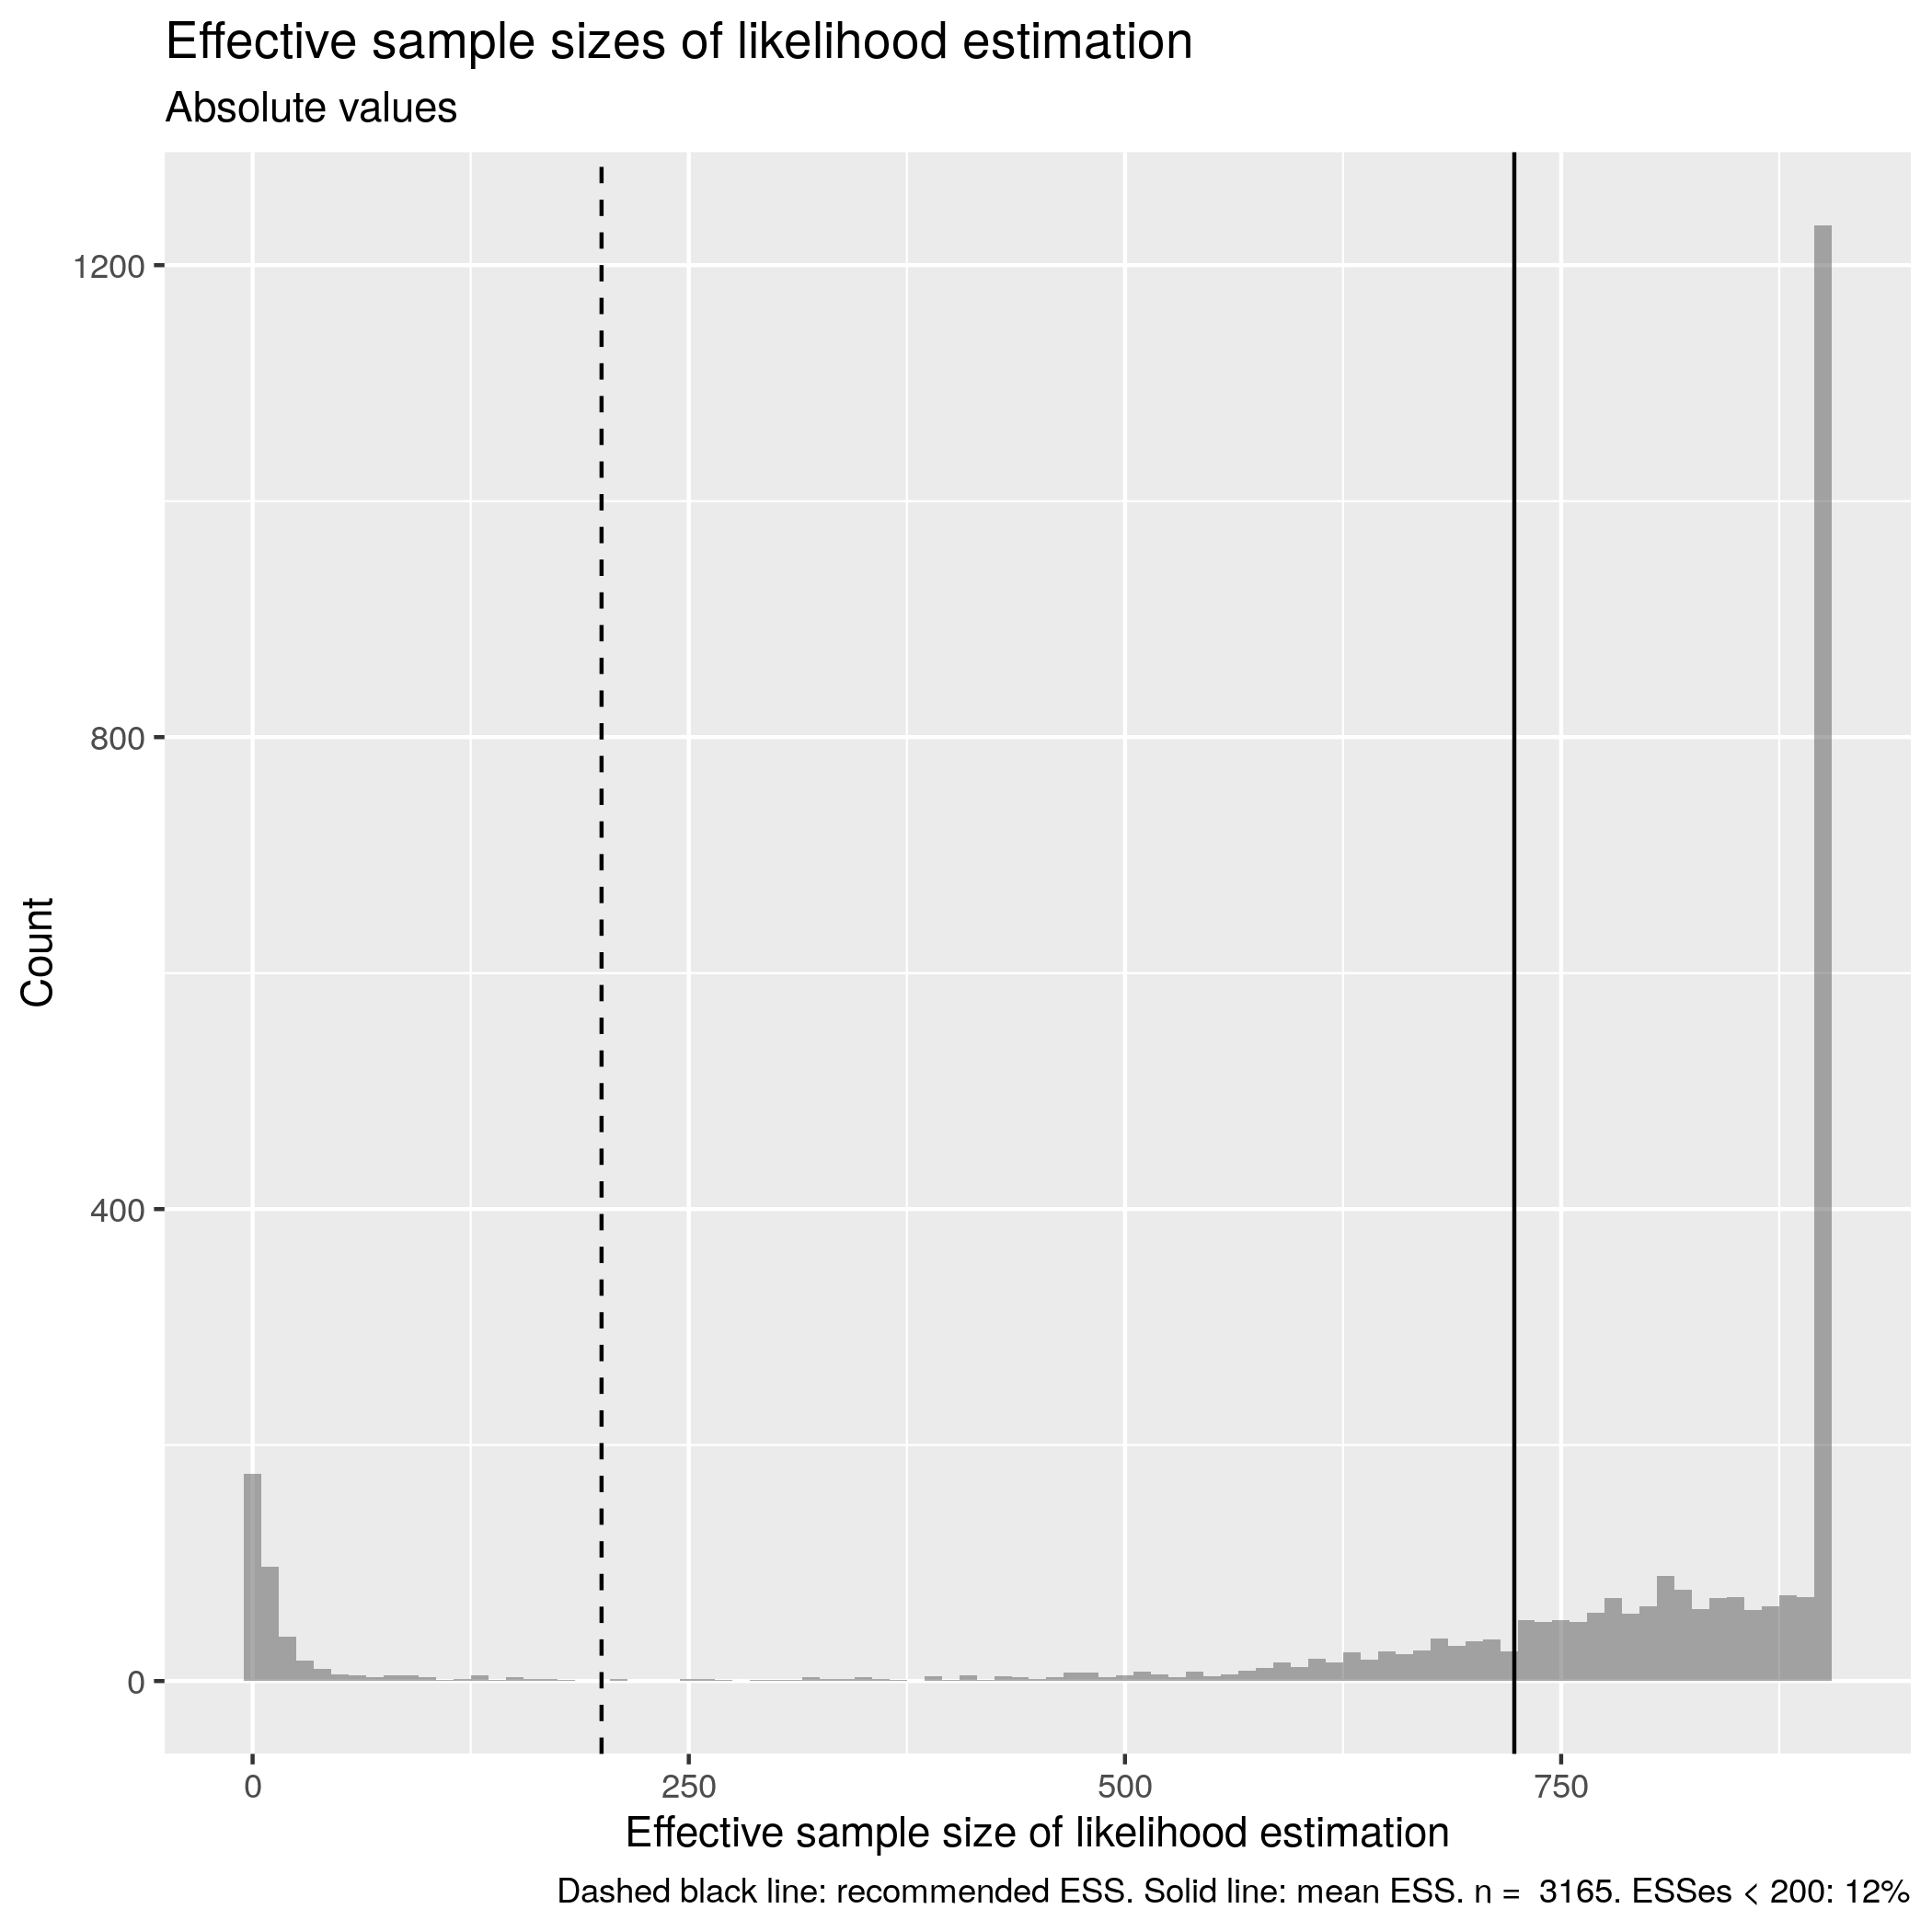
\includegraphics[width=\textwidth]{20200204_fig_esses.png}
  \caption{
    Effective sample sizes of the likelihood of all the experiments that
    finished within 10 days. 
    Each point is one parameter setting.
  }
  \label{fig:esses}
\end{figure}

\begin{figure}[!htbp]
  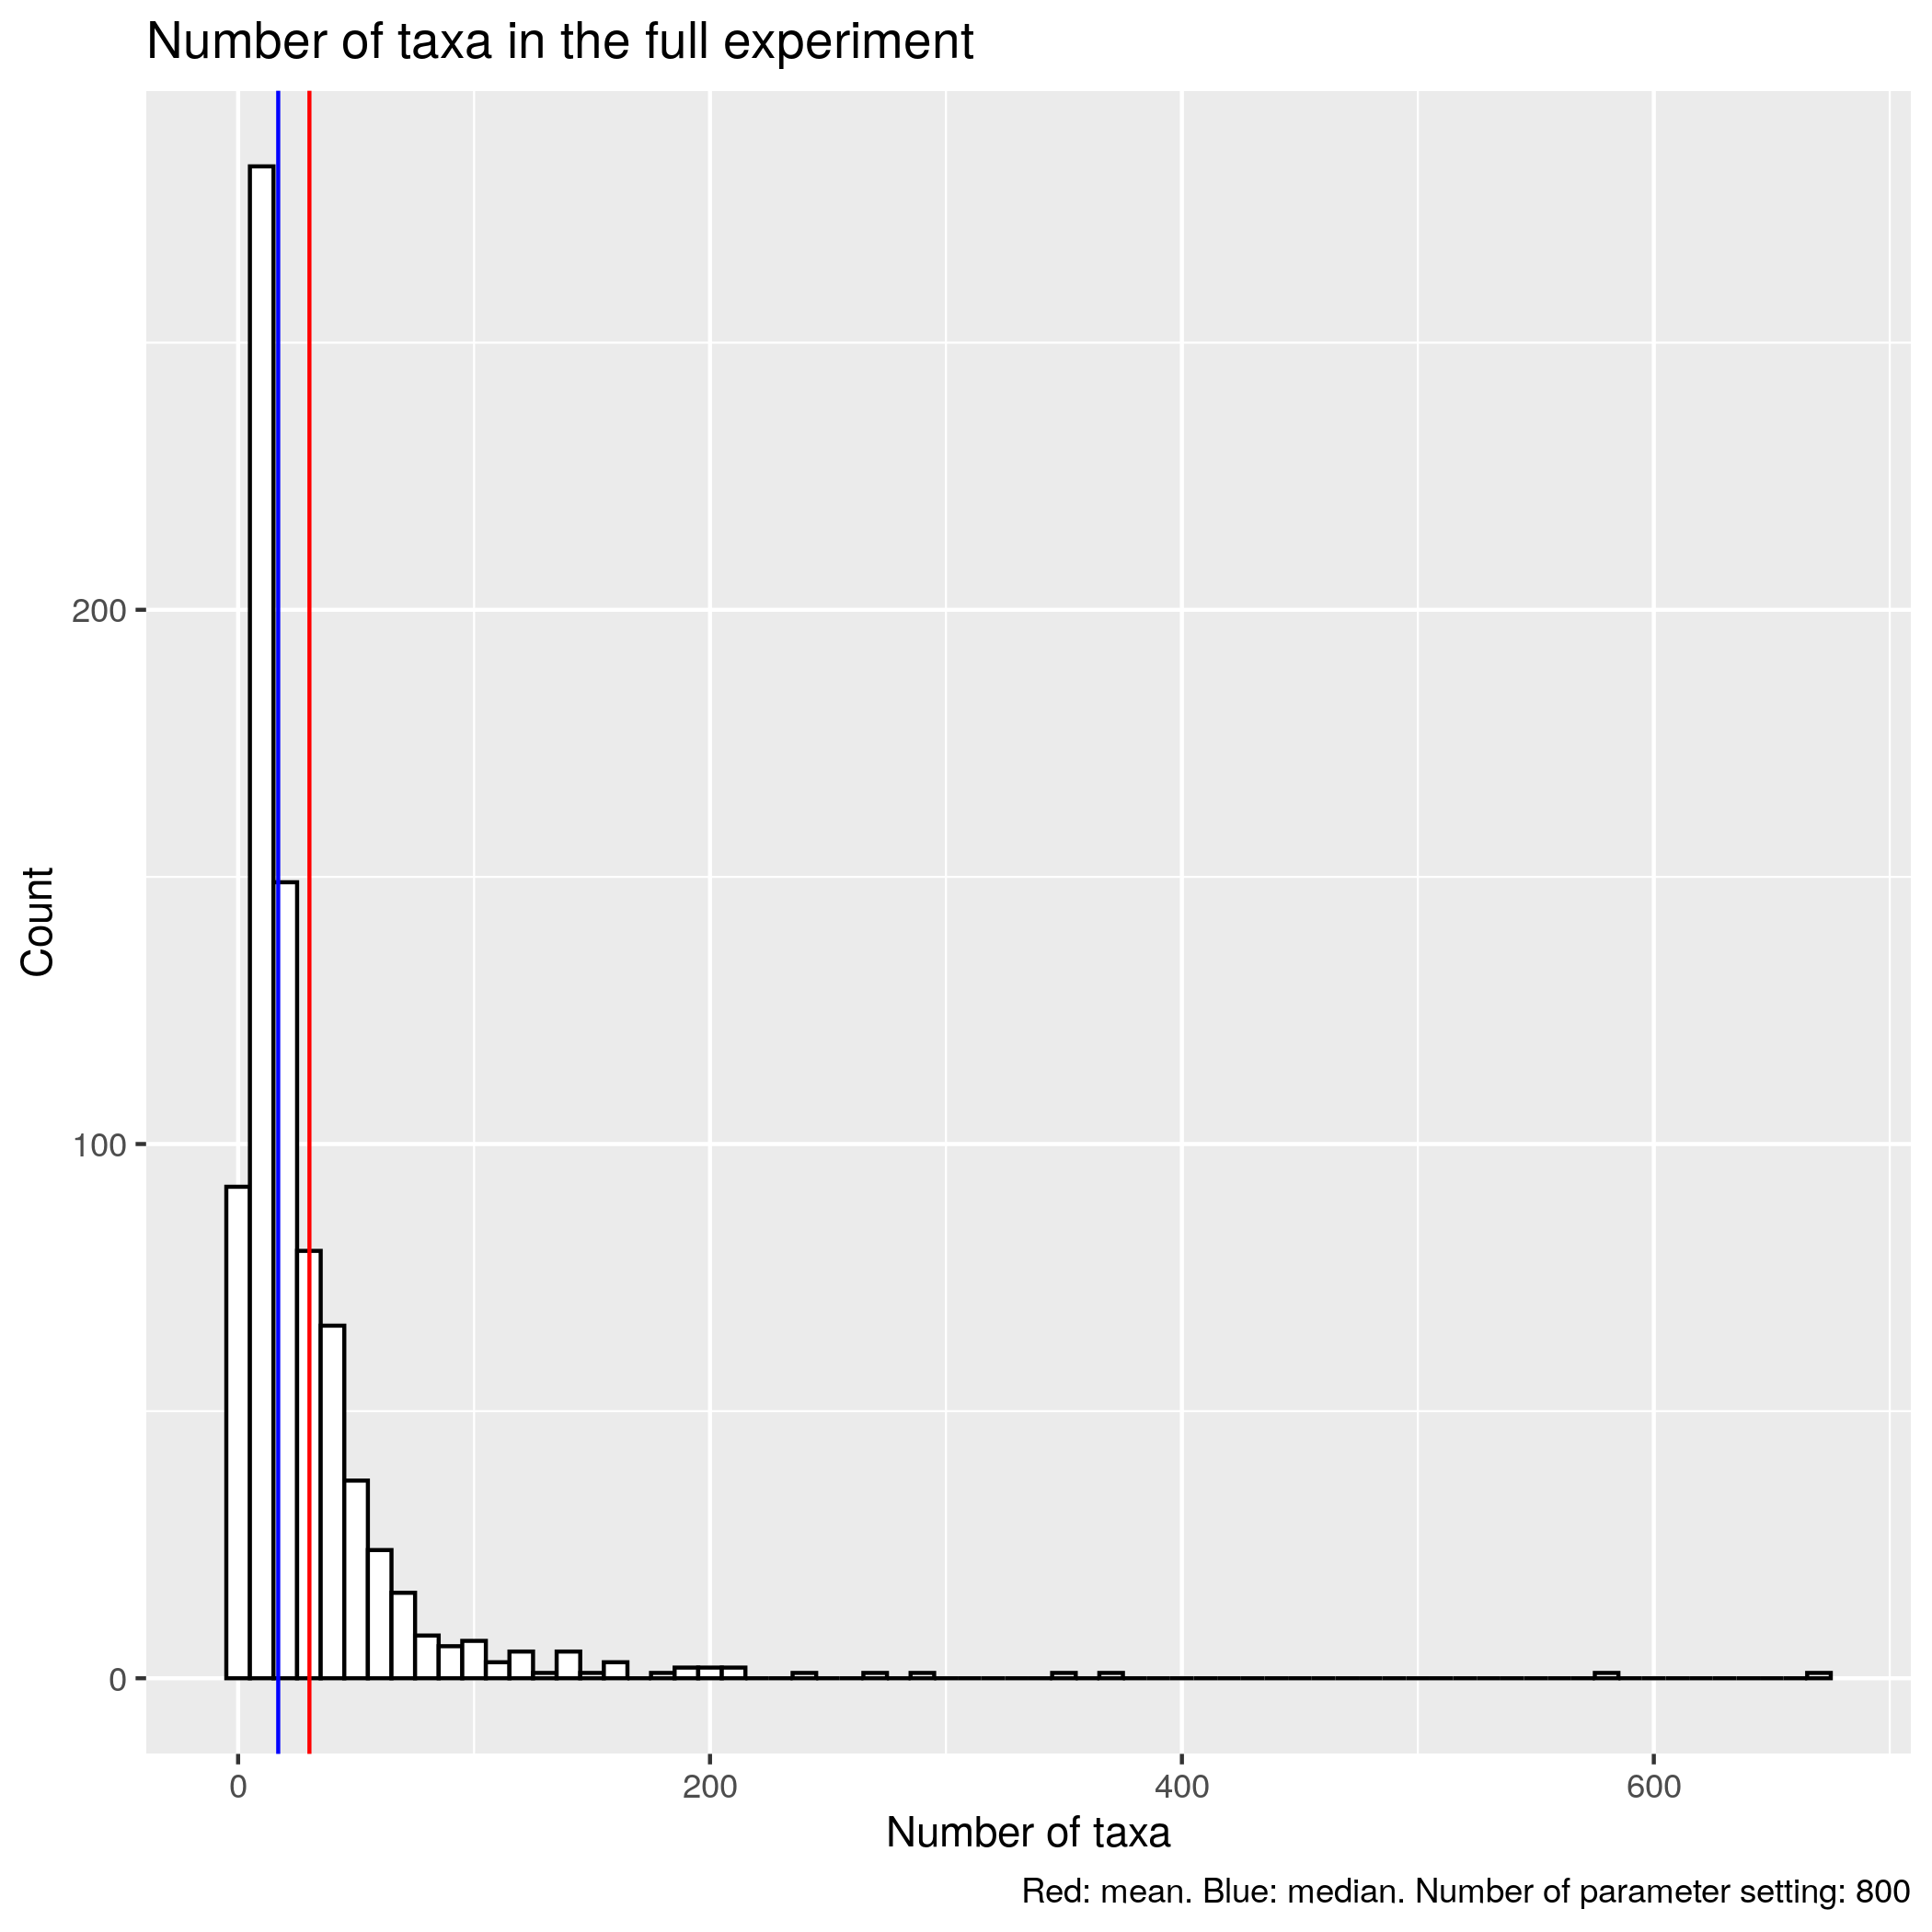
\includegraphics[width=\textwidth]{20200204_fig_n_taxa.png}
  \caption{
    Histogram of the number of taxa in the full experiment.
  }
  \label{fig:n_taxa}
\end{figure}

% 20200204_fig_marg_liks.png
% 20200204_fig_cumulative_esses.png
% 20200204_figure_1a.png
% 20200204_figure_1b.png
% 20200204_figure_1c.png
% 20200204_figure_1d.png

